\chapter{ws-Closed Sets and ws-Open Sets in Topological Spaces}
\graphicspath{{Chapter2/Chapter2Figs/EPS/}{Chapter2/Chapter2Figs/}}

N. Levine \cite{Levine} elaborated generalised closed sets in general topology as a generalisation of closed sets. This Knowledge of generalised closed sets was enhanced the improvisation of many new results in general topology. Many topologist namely Balachandran et al \cite{Balachandran}, Bhattacharya et al \cite{Bhattacharya}, Arockirani \cite{Arockiarani}, Gnanambal \cite{Gnanambal}, Malghan \cite{Malghan}, Devi \cite{Devi}, Benchalli \cite{Benchalli}, R.S. Walli \cite{Wali2} has contributed their works on generalised closed sets, their generalisation and related concept in general topology.

Second section describes a new class of closed sets known as weekly semi closed sets (ws-closed) in topological spaces which are explored and examined. During practise of study few properties of ws-closed sets are obtained and it was found that every semi-closed sets are ws-closed sets,

Third Section describes about a new class of open sets known as weekly semi open sets (ws-open) in topological spaces which are elaborated and examined. During practise of study few properties ws-open sets are obtained. We introduce ws-neighbourhood in topological spaces by using notations of ws-open sets. The notions of ws-interior, ws -closure are explored and studied with few of its basic properties and its basic results are obtained.

\section{ws-Closed sets and their basic properties}\label{sec}

\begin{dfn}\label{defi2.2.1}
A subset $\clrD$ of a space $(\TSP,\tau)$ is called ws-closed set if $\scl(\clrD) \subseteq \TSU$, whenever $\clrD\subseteq \TSU$ and $U$ is w-open in $(\TSP,\tau)$. We denote the collection of all ws-closed sets in $\TSP$ by $\mbox{WSC}(\TSP)$.
\end{dfn}

First we prove that the class ws-closed sets properly lies between the class all semi-closed sets and generalised semi pre-closed sets in topological spaces.

\begin{thm}\label{thm2.2.2}
Each semi-closed set in $\TSP$ is ws-closed set but inverse is untrue.
\end{thm}

\begin{proof}
Let $\clrD$ be semi-closed set in $\TSP$. Let $M$ be any w-open set in $\TSP$, s.t $\clrD\subseteq \TSM$. Since $\clrD$ is semi-closed, we have $\scl(\clrD) = \clrD \subseteq M$, we have  $\scl(\clrD) \subseteq M$.   Hence $\clrD$ is ws-closed set in $\TSP$.
\end{proof}

We use example \ref{exam2.2.3} to prove the inverse of  theorem is untrue. 

\begin{exm}\label{exam2.2.3}
Let $\TSP= \{1, 2, 3, 4\}$ and  $\tau= \{\TSP, \phi, \{1\}, \{2\},\{1, 2\}, \{1, 2, 3\}\}$ then the set $\clrD= \{1,2,3\}$ is ws-closed set but not semi-closed in $\TSP$.  
\end{exm}

\begin{thm}\label{thm2.2.4}
\begin{enumerate}[(i)]
\item If $\clrD\in\alpha$-$\TSC(\TSP)$ is ws-$\TSC(\TSP)$ but inverse is untrue.

\item If $\clrD\in \TSg^{\#}$-$\TSC(\TSP)$ is ws-$\TSC(\TSP)$ but inverse is untrue.

\item If $\clrD\in {}^{*}\TSg\alpha$-$\TSC(\TSP)$ is ws-$\TSC(\TSP)$ but inverse is untrue.

\item If $\clrD\in \TSg\# \TSs$-$\TSC(\TSP)$ is ws-$\TSC(\TSP)$ but inverse is untrue.

\item If $\clrD\in \TSg\xi$*-$\TSC(\TSP)$ is ws-$\TSC(\TSP)$ but inverse is untrue.

\item If $\clrD\in \alpha\TSg\TSp$-$\TSC(\TSP)$ is ws-$\TSC(\TSP)$ but inverse is untrue.

\item If $\clrD\in \ddot{g}$-$\TSC(\TSP)$ is ws-$\TSC(\TSP)$ but inverse is untrue.

\item If $\clrD\in$ regular-$\TSC(\TSP)$ is ws-$\TSC(\TSP)$ but inverse is untrue.

\item If $\clrD\in \TSr\TSb$-$\TSC(\TSP)$ is ws-$\TSC(\TSP)$ but inverse is untrue.
\end{enumerate}
\end{thm}

\begin{proof}
Let $\clrD$ be $\alpha$-(respectively, $\TSg\#$, $*\TSg\alpha$, $\TSg\# \TSs$, $\TSg\xi*$, $\alpha\TSg\TSp$, $\ddot{g}$ regular and $rb$) closed set in $\TSP$. Let $M$ be any w-open set in $\TSP$, s.t $\clrD \subseteq M$. Since $\clrD$ is $\alpha$- (respectively, $\TSg\#$, $*\TSg\alpha$, $g\# \TSs$, $g\xi^{*}$, $\alpha\TSg\TSp$, $\ddot{g}$, regular and rb) closed in $\TSP$, we have $\scl(\clrD) = \clrD \subseteq M$, we have $\scl(\clrD) \subseteq \TSM$. Hence $\clrD$ is ws-closed set in $\TSP$.
\end{proof}

\begin{exm}\label{exam2.2.5}
Let $\TSP= \{1, 2, 3, 4\}$ and $\tau=\{\TSP, \phi, \{1\}, \{2\},\{1, 2\}, \{1, 2, 3\}\}$ then the set $\clrD=\{1\}$ is ws-closed set but not $\alpha$- (respectively, $\TSg\#$, $*\TSg\alpha$, $\TSg\# \TSs$, $\TSg\xi^{*}$, $\alpha\TSg\TSp$, $\ddot{g}$, regular and rb) closed set in $\TSP$.
\end{exm}

\begin{thm}\label{thm2.2.6}
Each $\psi$-closed set in $\TSP$ is ws-closed set but inverse is untrue
\end{thm}

\begin{proof}
Let $\clrD$ be $\psi$-closed set in $\TSP$. Let $\TSM$ be any w-open set in $\TSP$, s.t $\clrD\subseteq \TSM$. Since $\clrD$ is $\psi$-closed, we have $\scl(\clrD)=\clrD\subseteq \TSM$, we have $\scl(\clrD)\subseteq \TSM$. Hence $\clrD$ is ws-closed set in $\TSP$.
\end{proof}

We use example \ref{exam2.2.7} to prove the inverse of theorem is untrue.

\begin{exm}\label{exam2.2.7}
Let $\TSP= \{1, 2, 3, 4\}$ and  $\tau= \{\TSP, \phi, \{1\}, \{2\},\{1, 2\}, \{1, 2, 3\}\}$ then the set $\clrD= \{1,2,3\}$ is ws-closed set but not $\psi$-closed in $\TSP$.
\end{exm}

\begin{coro}\label{coro2.2.8}
If $\clrD\in$ closed set is ws-$\TSC(\TSP)$ set in $\TSP$.
\end{coro}

\begin{proof}
Each closed set is $\alpha$-closed and follows from Theorem \ref{thm2.2.4}. Every $\alpha$-closed set is ws-closed set. Therefore Every closed set is ws-closed set in $\TSP$.
\end{proof}

We use example \ref{exam2.2.9} to prove the inverse of theorem is untrue. 

\begin{exm}\label{exam2.2.9}
Let $\TSP= \{1, 2, 3, 4\}$ and  $\tau= \{\TSP, \phi, \{1\}, \{2\}, \{1, 2\}, \{1, 2, 3\}\}$ then the set $\clrD = \{1\}$ is ws-closed set but not closed in $\TSP$.
\end{exm}

\begin{thm}\label{thm2.2.10}
If $\clrD\in \ws$-$\TSC(\TSP)$ is gspr-closed set in $\TSP$ but inverse is untrue.
\end{thm}

\begin{proof}
Take up $\clrD\in\ws$-$\TSC(\TSP)$, let $\TSM$ be any regular open set in $\TSP$ s.t $\clrD \subseteq \TSM$. Since each regular open set is w-open set and $\clrD$ is ws-closed set, we have $\scl(\clrD)\subseteq \TSM$,

Therefore $\scl(\clrD)\TSM$, $\TSM$ is regular open in $\TSP$, $\clrD$ is gspr-$\TSC(\TSP)$.
\end{proof}

We use example \ref{exam2.2.11} to prove the inverse of theorem is untrue.

\begin{exm}\label{exam2.2.11}
Let $\TSP = \{1, 2, 3 4\}$, $\tau = \{\TSP,\phi,\{1, 2\}, \{3, 4\}\}$. Then the set $\clrD= \{1\}$ is gspr-closed set but not ws-closed set in $\TSP$.
\end{exm}

\begin{coro}\label{coro2.2.12}
\begin{itemize}
\item[(i)] If $\clrD\in \ws$-$\TSC(\TSP)$ then $\clrD\in \gsp$-$\TSC(\TSP)$ but inverse is untrue.
\item[(ii)] If $\clrD\in \ws$-$\TSC(\TSP)$ $\clrD\in \rgb$-$\TSC(\TSP)$ but inverse is untrue.
\end{itemize}
\end{coro}

\begin{proof}
\begin{itemize}
\item[(i)] Follow from \cite{Navalagi2} Govindappa Navalagi, S.V. Gurushantanavar, and Chandrashekarappa A.S. Each gspr-$\TSC(\TSP)$ set is gsp-$\TSC(\TSP)$ set and then follows from Theorem \ref{thm2.1.4}.

\item[(ii)] Follow from [2013] K. Mariappa, S. Sekar, \cite{Mariappa} each rgb-closed is gsp-closedset, then follows from Corollary \ref{coro2.1.2}(i).
\end{itemize}
We use example \ref{exam2.2.13} to prove the inverse of above Corallary is untrue.
\end{proof}

\begin{exm}\label{exam2.2.13}
Let $\TSP = \{1, 2, 3, 4\}$, $\tau = \{\TSP, \phi, \{1, 2\}, \{3, 4\}\}$. Then the set $\clrD= \{2\}$ is gsp(rgb)-closed set but not ws-closed set in $\TSP$.
\end{exm}

\begin{rem}\label{rem2.2.14}
The following Examples shows that $\ws$-$\TSC(\TSP)$ sets are independent of $\rg$-$\TSC(\TSP)$ sets, $\gpr$-$\TSC(\TSP)$ sets, $\wgr\alpha$-$\TSC(\TSP)$ sets, $\pgr\alpha$-$\TSC(\TSP)$ sets, $\widehat{rg}\alpha$-$\TSC(\TSP)$ sets, $\alpha{*}{*}\TSg$-$\TSC(\TSP)$ sets, $\gprw$-$\TSC(\TSP)$ sets, $\rgw$-$\TSC(\TSP)$ sets, $\rw$-$\TSC(\TSP)$ sets, $\rwg$-$\TSC(\TSP)$ sets, $\rg\alpha$-$\TSC(\TSP)$ sets, $\alpha\gr$-$\TSC(\TSP)$ sets, $\TSg\alpha {*}{*}$-$\TSC(\TSP)$ sets, $\beta \wg{*}{*}$-$\TSC(\TSP)$ sets.
\end{rem}

\begin{exm}\label{exm2.2.15}
Let $\TSP = \{1, 2, 3, 4\}$, $\tau = \{\TSP,\phi, \{1\}, \{2\}, \{1, 2\}, \{1, 2, 3\}\}$. Then 
\begin{enumerate}[(i)]
\item Closed sets in $(\TSP, \tau)$ are $\TSP$, $\phi$, $\{4\}$, $\{3, 4\}$, $\{1, 3, 4\}$, $\{2, 3, 4\}$.

\item ws-Closed in $(\TSP, \tau)$ are $\TSP$, $\phi$, $\{1\}$, $\{2\}$, $\{3\}$, $\{4\}$, $\{1, 3\}$, $\{1, 4\}$, $\{2, 3\}$, $\{2, 4\}$, $\{3, 4\}$, $\{1, 2, 4\}$, $\{1, 3, 4\}$, $\{2, 3, 4\}$.

\item rg-Closed in $(\TSP, \tau)$ are $\TSP$, $\phi$, $\{3\}$, $\{4\}$, $\{1, 2\}$, $\{1, 3\}$, $\{1 4\}$, $\{2, 3\}$, $\{2, 4\}$, $\{3, 4\}$, $\{1, 2, 3\}$, $\{1, 2, 4\}$, $\{1, 3, 4\}$, $\{2, 3, 4\}$.

\item gpr-Closed in $(\TSP, \tau)$ are $\TSP$, $\phi$, $\{3\}$, $\{4\}$, $\{1, 2\}$, $\{1, 3\}$, $\{1 4\}$, $\{2, 3\}$, $\{2, 4\}$, $\{3, 4\}$, $\{1, 2, 3\}$, $\{1, 2, 4\}$, $\{1, 3, 4\}$, $\{2, 3, 4\}$.

\item wgr$\alpha$-Closed in $(\TSP, \tau)$ are $\TSP$, $\phi$, $\{3\}$, $\{4\}$, $\{1, 2\}$, $\{1, 3\}$, $\{1 4\}$, $\{2, 3\}$, $\{2, 4\}$, $\{3, 4\}$, $\{1, 2, 3\}$, $\{1, 2, 4\}$, $\{1, 3, 4\}$, $\{2, 3, 4\}$.

\item pgr$\alpha$-Closed in $(\TSP, \tau)$ are $\TSP$, $\phi$, $\{3\}$, $\{4\}$, $\{1, 2\}$, $\{1, 3\}$, $\{1 4\}$, $\{2, 3\}$, $\{2, 4\}$, $\{3, 4\}$, $\{1, 2, 3\}$, $\{1, 2, 4\}$, $\{1, 3, 4\}$, $\{2, 3, 4\}$.

\item $\widehat{rg}$-Closed in $(\TSP, \tau)$ are $\TSP$, $\phi$, $\{3\}$, $\{4\}$, $\{1, 2\}$, $\{1, 3\}$, $\{1 4\}$, $\{2, 3\}$, $\{2, 4\}$, $\{3, 4\}$, $\{1, 2, 3\}$, $\{1, 2, 4\}$, $\{1, 3, 4\}$, $\{2, 3, 4\}$.

\item $\alpha{*}{*} g$-Closed in $(\TSP, \phi)$ are $\TSP$, $\phi$, $\{3\}$, $\{4\}$, $\{1, 2\}$, $\{1, 3\}$, $\{1 4\}$, $\{2, 3\}$, $\{2, 4\}$, $\{3, 4\}$, $\{1, 2,3\}$, $\{1, 2, 4\}$, $\{1, 3, 4\}$, $\{2, 3, 4\}$.

\item gprw-Closed in $(\TSP, \tau)$ are $\TSP$, $\phi$, $\{3\}$, $\{4\}$, $\{1, 2\}$, $\{3, 4\}$, $\{1, 2, 3\}$, $\{1, 2, 4\}$, $\{1, 3, 4\}$, $\{2, 3,4\}$.

\item rgw-Closed in $(\TSP, \tau)$ are $\TSP$, $\phi$, $\{3\}$, $\{4\}$, $\{1, 2\}$, $\{3, 4\}$, $\{1, 2, 3\}$, $\{1, 2, 4\}$, $\{1, 3, 4\}$, $\{2, 3, 4\}$.

\item rw-Closed in $(\TSP, \tau)$ are $\TSP, \phi,\{4\},\{1, 2\},\{3, 4\},\{1, 2, 3\},\{1, 2, 4\},\{1, 3, 4\},\{2, 3, 4\}$.

\item rwg-Closed in $(\TSP, \tau)$ are $\TSP$, $ \phi$, $\{1\}$, $\{2\}$, $\{3\}$, $\{4\}$, $\{1,  3\}$, $\{1, 4\}$, $\{2, 3\}$, $\{2, 4\}$, $\{3, 4\}$, $\{1, 2, 4\}$, $\{1, 3, 4\}$, $\{2, 3, 4\}$.

\item rg$\alpha$-Closed in $(\TSP, \tau)$ are $\TSP$, $ \phi$, $\{1\}$, $\{2\}$, $\{3\}$, $\{4\}$, $\{1, 3\}$, $\{1, 4\}$, $\{2, 3\}$, $\{2, 4\}$, $\{3, 4\}$, $ \{1, 2, 4\}$, $ \{1, 3, 4\}$, $\{2, 3, 4\}$.

\item $\alpha$gr-Closed in $(\TSP, \tau)$ are $\TSP$, $ \phi$, $\{1\}$, $\{2\}$, $\{3\}$, $\{4\}$, $\{1, 3\}$, $\{1, 4\}$, $\{2, 3\}$, $\{2, 4\}$, $\{3, 4\}$, $ \{1, 2, 4\}$, $ \{1, 3, 4\}$, $\{2, 3, 4\}$.

\item $\TSg\alpha {*}{*}$-Closed in $(\TSP, \tau)$ are $\TSP$, $ \phi$, $\{1\}$, $\{2\}$, $\{3\}$, $\{4\}$, $\{1, 3\}$, $\{1, 4\}$, $\{2, 3\}$, $\{2, 4\}$, $\{3, 4\}$, $ \{1, 2, 4\}$, $ \{1, 3, 4\}$, $\{2, 3, 4\}$.

\item $\beta \wg{*}{*}$-Closed in $(\TSP, \tau)$ are $\TSP$, $ \phi$, $\{1\}$, $\{2\}$, $\{3\}$, $\{4\}$, $\{1, 3\}$, $\{1, 4\}$, $\{2, 3\}$, $\{2, 4\}$, $\{3, 4\}$, $ \{1, 2, 4\}$, $ \{1, 3, 4\}$, $\{2, 3, 4\}$.
\end{enumerate}
\end{exm}

Therefore $\{1\}$ is ws-closed in $\TSP$ but not rg (resp. gpr, wgr$\alpha$, pgr$\alpha$, $\widehat{rg}$, $\alpha${*}{*}$\TSg$, gprw, rgw, rw, rwg, rg$\alpha$, $\alpha$gr, g$\alpha${*}{*} $\beta \wg${*}{*}) closed set in $\TSP$.

\begin{rem}\label{rem2.2.16}
The following examples clearly represent that ws-closed sets are independent of sets. *g, Mildly g, wg, gw$\alpha$, g*p, $\eta$, gp, $\beta$wg*, {*}{*}g$\alpha$, $\hat{g}$, $\tilde{g}$, $\alpha$gs, w$\alpha\hat{g}$-, $\#$g$\alpha$, og$\#$, g*-pre and g\#p\#, g$\alpha$*, $\alpha$g, g{*}{*}) closed sets.
\end{rem}

\begin{exm}\label{exm2.2.17}
Let $\TSP = \{1, 2, 3\}$, $\tau_{1} = \{\TSP, \phi, \{1\}, \{2\}, \{1, 2\}\}$ and $\tau_{2} = \{\TSP, \phi, \{1\},\break \{2, 3\}\}$. Then
\begin{enumerate}[(i)]
\item closed sets in $(\TSP, \tau_{1})$ are $\TSP$, $\phi$, $\{3\}$, $\{1, 3\}$, $\{2, 3\}$.
\item ws-closed sets $\in(\TSP, \tau_{1})$ are $\TSP$, $\phi$, $\{1\}$, $\{2\}$, $\{3\}$, $\{1, 3\}$, $\{2, 3\}$.
\item *g-closed sets $\in(\TSP, \tau_{1})$ are $\TSP$, $\phi$, $\{3\}$, $\{1, 3\}$, $\{2, 3\}$.
\item Mildly g-closed sets $\in(\TSP, \tau_{1})$ are $\TSP$, $\phi$, $\{3\}$, $\{1, 3\}$, $\{2, 3\}$.
\item wg-closed sets $\in(\TSP, \tau_{1})$ are $\TSP$, $\phi$, $\{3\}$, $\{1, 3\}$, $\{2, 3\}$.
\item gw$\alpha$-closed sets $\in(\TSP, \tau_{1})$ are $\TSP$, $\phi$, $\{3\}$, $\{1, 3\}$, $\{2, 3\}$.
\item g*p-closed sets $\in(\TSP, \tau_{1})$ are $\TSP$, $\phi$, $\{3\}$, $\{1, 3\}$, $\{2, 3\}$.
\item $\eta$-closed sets $\in(\TSP, \tau_{1})$ are $\TSP$, $\phi$, $\{3\}$, $\{1, 3\}$, $\{2, 3\}$.
\item gp-closed sets $\in(\TSP, \tau_{1})$ are $\TSP$, $\phi$, $\{3\}$, $\{1, 3\}$, $\{2, 3\}$.
\item $\beta$wg*-closed sets $\in(\TSP, \tau_{1})$ are $\TSP$, $\phi$, $\{3\}$, $\{1, 3\}$, $\{2, 3\}$.
\item {*}{*}g$\alpha$-closed sets $\in(\TSP, \tau_{1})$ are $\TSP$, $\phi$, $\{3\}$, $\{1, 3\}$, $\{2, 3\}$.
\item $\hat{g}$-closed sets $\in(\TSP, \tau_{1})$ are $\TSP$, $\phi$, $\{3\}$, $\{1, 3\}$, $\{2, 3\}$.
\item $\tilde{g}$-closed sets $\in(\TSP, \tau_{1})$ are $\TSP$, $\phi$, $\{3\}$, $\{1, 3\}$, $\{2, 3\}$.
\item $\alpha$gs-closed sets $\in(\TSP, \tau_{1})$ are $\TSP$, $\phi$, $\{3\}$, $\{1, 3\}$, $\{2, 3\}$.
\item \#g$\alpha$-closed sets $\in(\TSP, \tau_{1})$ are $\TSP$, $\phi$, $\{3\}$, $\{1, 3\}$, $\{2, 3\}$.
\item g*-pre closed sets $\in(\TSP, \tau_{1} )$ are $\TSP$, $\phi$, $\{3\}$, $\{1, 3\}$, $\{2, 3\}$.
\item g\#p\#-closed sets $\in(\TSP, \tau_{1} )$ are $\TSP$, $\phi$, $\{3\}$, $\{1, 3\}$, $\{2, 3\}$.
\item g$\alpha$*-closed sets $\in(\TSP, \tau_{1} )$ are $\TSP$, $\phi$, $\{3\}$, $\{1, 3\}$, $\{2, 3\}$.
\item $\alpha$g-closed sets $\in(\TSP, \tau_{1})$ are $\TSP$, $\phi$, $\{3\}$, $\{1, 3\}$, $\{2, 3\}$.
\item g{*}{*}-closed sets $\in(\TSP, \tau_{1})$ are $\TSP$, $\phi$, $\{3\}$, $\{1, 3\}$, $\{2, 3\}$. and also
\end{enumerate}

\begin{enumerate}[(i)]
\item closed sets $\in(\TSP, \tau_{2})$ are $\TSP$, $\phi$, $\{1\}$, $\{2, 3\}$.
\item ws-closed sets $\in(\TSP, \tau_{2})$ are $\TSP$, $\phi$, $\{1\}$, $\{2, 3\}$.
\item *g-closed sets $\in(\TSP, \tau_{2})$ are $\TSP$, $\phi$, $\{1\}$, $\{2\}$, $\{3\}$, $\{1, 2\}$, $\{1, 3\}$, $\{2, 3\}$.
\item Mildly g-closed sets $\in(\TSP, \tau_{2})$ are $\TSP$, $\phi$, $\{1\}$, $\{2\}$, $\{3\}$, $\{1, 2\}$, $\{1, 3\}$, $\{2, 3\}$.
\item wg-closed sets $\in(\TSP, \tau_{2})$ are $\TSP$, $\phi$, $\{1\}$, $\{2\}$, $\{3\}$, $\{1, 2\}$, $\{1, 3\}$, $\{2, 3\}$.
\item gw$\alpha$-closed sets $\in(\TSP, \tau_{2})$ are $\TSP$, $\phi$, $\{1\}$, $\{2\}$, $\{3\}$, $\{1, 2\}$, $\{1, 3\}$, $\{2, 3\}$.
\item g*p-closed sets $\in(\TSP, \tau_{2})$ are $\TSP$, $\phi$, $\{1\}$, $\{2\}$, $\{3\}$, $\{1, 2\}$, $\{1, 3\}$, $\{2, 3\}$.
\item $\eta$-closed sets $\in(\TSP, \tau_{2})$ are $\TSP$, $\phi$, $\{1\}$, $\{2\}$, $\{3\}$, $\{1, 2\}$, $\{1, 3\}$, $\{2, 3\}$.
\item gp-closed sets $\in(\TSP, \tau_{2})$ are $\TSP$, $\phi$, $\{1\}$, $\{2\}$, $\{3\}$, $\{1, 2\}$, $\{1, 3\}$, $\{2, 3\}$.
\item $\beta$wg*-Closed in $(\TSP, \tau_{2})$ are $\TSP$, $\phi$, $\{1\}$, $\{2\}$, $\{3\}$, $\{1, 2\}$, $\{1, 3\}$, $\{2, 3\}$.
\item {*}{*}g$\alpha$-closed sets $\in(\TSP, \tau_{2})$ are $\TSP$, $\phi$, $\{1\}$, $\{2\}$, $\{3\}$, $\{1, 2\}$, $\{1, 3\}$, $\{2, 3\}$.
\item $\hat{g}$-closed sets $\in(\TSP, \tau_{2})$ are $\TSP$, $\phi$, $\{1\}$, $\{2\}$, $\{3\}$, $\{1, 2\}$, $\{1, 3\}$, $\{2, 3\}$.
\item $\tilde{g}$-closed sets $\in(\TSP, \tau_{2})$ are $\TSP$, $\phi$, $\{1\}$, $\{2\}$, $\{3\}$, $\{1, 2\}$, $\{1, 3\}$, $\{2, 3\}$.
\item $\alpha$gs-closed sets $\in(\TSP, \tau_{2})$ are $\TSP$, $\phi$, $\{1\}$, $\{2\}$, $\{3\}$, $\{1, 2\}$, $\{1, 3\}$, $\{2, 3\}$.
\item \#g$\alpha$-closed sets $\in(\TSP, \tau_{2})$ are $\TSP$, $\phi$, $\{1\}$, $\{2\}$, $\{3\}$, $\{1, 2\}$, $\{1, 3\}$, $\{2, 3\}$.
\item g*-pre closed sets $\in(\TSP, \tau_{2})$ are $\TSP$, $\phi$, $\{1\}$, $\{2\}$, $\{3\}$, $\{1, 2\}$, $\{1, 3\}$, $\{2, 3\}$.
\item g\#p\#-closed sets $\in(\TSP, \tau_{2})$ are $\TSP$, $\phi$, $\{1\}$, $\{2\}$, $\{3\}$, $\{1, 2\}$, $\{1, 3\}$, $\{2, 3\}$.
\item g$\alpha$*-closed sets $\in(\TSP, \tau_{2})$ are $\TSP$, $\phi$, $\{1\}$, $\{2\}$, $\{3\}$, $\{1, 2\}$, $\{1, 3\}$, $\{2, 3\}$.
\item $\alpha$g-closed sets $\in(\TSP, \tau_{2})$ are $\TSP$, $\phi$, $\{1\}$, $\{2\}$, $\{3\}$, $\{1, 2\}$, $\{1, 3\}$, $\{2, 3\}$.
\item g{*}{*}-closed sets $\in(\TSP, \tau_{2})$ are $\TSP$, $\phi$, $\{1\}$, $\{2\}$, $\{3\}$, $\{1, 2\}$, $\{1, 3\}$, $\{2, 3\}$.
\end{enumerate}

Therefore $\{2\}$ is ws-closed set in $(\TSP, \tau_{1})$ but not in *g (resp. Mildly g, wg, gw$\alpha$, g*p, $\eta$, gp, $\beta$wg*, {*}{*}g$\alpha$, $\hat{g}$, $\tilde{g}$, $\alpha$gs, $\alpha\hat{g}$, \#g$\alpha$, og\#, g*-pre, g\#p\#, g$\alpha$*, $\alpha$g, g{*}{*})$\TSC(\TSP)$ set in $(\TSP,\tau_{1})$.

Meanwhile $\{2\}$ in *g-(resp. gw$\alpha$, g*p, $\eta$, gp, $\beta$wg*, {*}{*}g$\alpha$, $\hat{g}$, $\tilde{g}$, $\alpha$gs, $\alpha\hat{g}$, \#g$\alpha$, og\#, g*-pre, g\#p\#, g$\alpha$*, $\alpha$g, g{*}{*})$\TSC(\TSP)$ in $(\TSP, \tau_{2})$ but not ws-$\TSC(\TSP)$ set in $(\TSP, \tau_{2})$.
\end{exm}

\begin{rem}\label{rem2.2.18}
The following example clearly represents that ws-closed sets are independent of sets g, sg, gs, g$\alpha$, sgb, rg*b, pgpr, g$\alpha$b and rps-closed sets in $\TSP$.
\end{rem}

\begin{exm}\label{exm2.2.19}
Let $\TSP = \{1, 2, 3, 4\}$, $\tau_{1} =\{\TSP, \phi, \{1\}, \{1, 2\},\{1, 2, 3\}\}$ and $\tau_{2} =\{\TSP, \phi, \{1, 2\},\{3, 4\}\}$. Then
\begin{enumerate}[(i)]
\item closed sets $\in$ in $(\TSP, \tau_{1})$ are $\TSP$, $\phi$, $\{4\}$, $\{3, 4\}$, $\{2, 3, 4\}$.
\item ws-closed sets $\in(\TSP, \tau_{1})$ are $\TSP$, $\phi$, $\{1\}$, $\{2\}$, $\{3\}$, $\{4\}$, $\{1, 3\}$, $\{1, 4\}$, $\{2, 3\}$, $\{2, 4\}$, $\{3, 4\}, \{1, 2, 4\}, \{1, 3, 4\}$, $\{2, 3, 4\}$.
\item g-closed sets $\in(\TSP, \tau_{1})$ are $\TSP$, $\phi$, $\{4\}$, $\{1, 4\}$, $\{2, 4\}$, $\{3, 4\}$, $\{1, 2, 4\}$, $\{1, 3, 4\}$, $\{2, 3, 4\}$.
\item sg-closed sets $\in(\TSP, \tau_{1})$ are $\TSP$, $\phi$, $\{2\}$, $\{3\}$, $\{4\}$, $\{2, 3\}$, $\{2, 4\}$, $\{3, 4\}$, $\{2, 3, 4\}$.
\item gs-closed sets $\in(\TSP, \tau_{1})$ are $\TSP$, $\phi$, $\{2\}$, $\{3\}$, $\{4\}$, $\{2, 3\}$, $\{2, 4\}$, $\{3, 4\}$, $\{2, 3, 4\}$.
\item g$\alpha$-closed sets $\in(\TSP, \tau_{1})$ are $\TSP$, $\phi$, $\{2\}$, $\{3\}$, $\{4\}$, $\{2, 3\}$, $\{2, 4\}$, $\{3, 4\}$, $\{2, 3, 4\}$.
\item sgb-closed sets $\in(\TSP, \tau_{1})$ are $\TSP$, $\phi$, $\{2\}$, $\{3\}$, $\{4\}$, $\{2, 3\}$, $\{2, 4\}$, $\{3, 4\}$, $\{2, 3, 4\}$.
\item rg*b-closed sets $\in(\TSP, \tau_{1})$ are $\TSP$, $\phi$, $\{2\}$, $\{3\}$, $\{4\}$, $\{2, 3\}$, $\{2, 4\}$, $\{3, 4\}$, $\{2, 3, 4\}$.
\item pgpr-closed sets $\in(\TSP, \tau_{1})$ are $\TSP$, $\phi$, $\{2\}$, $\{3\}$, $\{4\}$, $\{2, 3\}$, $\{2, 4\}$, $\{3, 4\}$, $\{2, 3, 4\}$.
\item g$\alpha$b-closed sets $\in(\TSP, \tau_{1})$ are $\TSP$, $\phi$, $\{2\}$, $\{3\}$, $\{4\}$, $\{2, 3\}$, $\{2, 4\}$, $\{3, 4\}$, $\{2, 3, 4\}$.
\item rps-closed sets $\in(\TSP, \tau_{1})$ are $\TSP$, $\phi$, $\{2\}$, $\{3\}$, $\{4\}$, $\{2, 3\}$, $\{2, 4\}$, $\{3, 4\}$, $\{2, 3, 4\}$. and also
\end{enumerate}

\begin{enumerate}[(i)]
\item Closed sets $\in(\TSP, \tau_{2})$ are $\TSP$, $\phi$, $\{3, 4\}$, $\{1, 2\}$.
\item ws-closed sets $\in(\TSP, \tau_{2})$ are $\TSP$, $\phi$, $\{1, 2\}$, $\{3, 4\}$.
\item g-closed sets $\in(\TSP, \tau_{2})$ are $\TSP$, $\phi$, $\{1\}$, $\{2\}$, $\{3\}$, $\{4\}$, $\{1, 2\}$, $\{1, 3\}$, $\{1, 4\}$, $\{2, 3\}$, $\{2, 4\}, \{3, 4\}$, $\{1, 2, 3\}$, $\{1, 2, 4\}$, $\{1, 3, 4\}$, $\{2, 3, 4\}$.
\item sg-closed sets $\in(\TSP, \tau_{2})$ are $\TSP$, $\phi$, $\{1\}$, $\{2\}$, $\{3\}$, $\{4\}$, $\{1, 2\}$, $\{1, 3\}$, $\{1, 4\}$, $\{2, 3\}$, $\{2, 4\}, \{3, 4\}$, $\{1, 2, 3\}$, $\{1, 2, 4\}$, $\{1, 3, 4\}$, $\{2, 3, 4\}$.
\item gs-closed sets $\in(\TSP, \tau_{2})$ are $\TSP$, $\phi$, $\{1\}$, $\{2\}$, $\{3\}$, $\{4\}$, $\{1, 2\}$, $\{1, 3\}$, $\{1, 4\}$, $\{2, 3\}$, $\{2, 4\}, \{3, 4\}$, $\{1, 2, 3\}$, $\{1, 2, 4\}$, $\{1, 3, 4\}$, $\{2, 3, 4\}$.
\item g$\alpha$-closed sets $\in(\TSP, \tau_{2})$ are $\TSP$, $\phi$, $\{1\}$, $\{2\}$, $\{3\}$, $\{4\}$, $\{1, 2\}$, $\{1, 3\}$, $\{1, 4\}$, $\{2, 3\}$, $\{2, 4\}, \{3, 4\}$, $\{1, 2, 3\}$, $\{1, 2, 4\}$, $\{1, 3, 4\}$, $\{2, 3, 4\}$.
\item sgb-closed sets $\in(\TSP, \tau_{2})$ are $\TSP$, $\phi$, $\{1\}$, $\{2\}$, $\{3\}$, $\{4\}$, $\{1, 2\}$, $\{1, 3\}$, $\{1, 4\}$, $\{2, 3\}$, $\{2, 4\}, \{3, 4\}$, $\{1, 2, 3\}$, $\{1, 2, 4\}$, $\{1, 3, 4\}$, $\{2, 3, 4\}$.
\item rg*b-closed sets $\in(\TSP, \tau_{2})$ are $\TSP$, $\phi$, $\{1\}$, $\{2\}$, $\{3\}$, $\{4\}$, $\{1, 2\}$, $\{1, 3\}$, $\{1, 4\}$, $\{2, 3\}$, $\{2, 4\}, \{3, 4\}$, $\{1, 2, 3\}$, $\{1, 2, 4\}$, $\{1, 3, 4\}$, $\{2, 3, 4\}$.
\item pgpr-closed sets $\in(\TSP, \tau_{2})$ are $\TSP$, $\phi$, $\{1\}$, $\{2\}$, $\{3\}$, $\{4\}$, $\{1, 2\}$, $\{1, 3\}$, $\{1, 4\}$, $\{2, 3\}$, $\{2, 4\}, \{3, 4\}$, $\{1, 2, 3\}$, $\{1, 2, 4\}$, $\{1, 3, 4\}$, $\{2, 3, 4\}$.
\item g$\alpha$b-closed sets $\in(\TSP, \tau_{2})$ are $\TSP$, $\phi$, $\{1\}$, $\{2\}$, $\{3\}$, $\{4\}$, $\{1, 2\}$, $\{1, 3\}$, $\{1, 4\}$, $\{2, 3\}$, $\{2, 4\}, \{3, 4\}$, $\{1, 2, 3\}$, $\{1, 2, 4\}$, $\{1, 3, 4\}$, $\{2, 3, 4\}$.
\item rps-closed sets $\in(\TSP, \tau_{2})$ are $\TSP$, $\phi$, $\{1\}$, $\{2\}$, $\{3\}$, $\{4\}$, $\{1, 2\}$, $\{1, 3\}$, $\{1, 4\}$, $\{2, 3\}$, $\{2, 4\}, \{3, 4\}$, $\{1, 2, 3\}$, $\{1, 2, 4\}$, $\{1, 3, 4\}$, $\{2, 3, 4\}$.
\end{enumerate}

Therefore $\{1\}$ is ws-$\TSC(\TSP)$ set in $(\TSP, \tau_{1})$ but not g-$\TSC(\TSP)$ (resp. sg-$\TSC(\TSP)$, gs-$\TSC(\TSP)$, g$\alpha$-$\TSC(\TSP)$, sgb-$\TSC(\TSP)$ sets, rg*b-$\TSC(\TSP)$, pgpr-$\TSC(\TSP)$, g$\alpha$b-$\TSC(\TSP)$, rps-$\TSC(\TSP)$) set in $(\TSP, \tau_{1})$.

Meanwhile $\{1\}$ is g-(resp. sg, gs, g$\alpha$, sgb, rg*b, pgpr, g$\alpha$b, rps) closed set in $(\TSP, \tau_{2})$ but not ws-closed set in $(\TSP, \tau_{2})$.
\end{exm}

\begin{rem}\label{rem2.2.20}
The next example represents that ws-closed will be independent of R*-closed set in $\TSX$.
\end{rem}

\begin{exm}\label{exm2.2.21}
Let $\TSX=\{1,2,3\}$, and $\tau=\{\TSX,\phi,\{1\},\{2\},\{1,2\}\}$. Then
\begin{enumerate}[(i)]
\item closed sets $\in(\TSX, \tau)$ are $\TSX, \phi,\{3\},\{1, 3\},\{2, 3\}$.
\item ws-$\TSC(\TSX)$ are $\TSX, \phi, \{1\},\{2\},\{3\},\{2, 3\}, \{1, 3\}$.
\item R*-$\TSC(\TSX)$ are $\TSX, \phi,\{3\},\{1, 2\},\{2, 3\},\{1, 3\}$.
\end{enumerate}

Therefore $\{1\}$ is ws-$\TSC(\TSX)$ set in $\TSX$ but not R* closed set in $\TSX$.
\end{exm}

\begin{exm}\label{add-exm2.2.21}
Let $\TSX=\{1,2,3\}$, and $\tau=\{\TSX,\phi,\{1\},\{2,3\}\}$. Then
\begin{enumerate}[(i)]
\item closed sets $\in(\TSX, \tau)$ are $\TSX, \phi,\{1\},\{2, 3\}$.
\item ws-$\TSC(\TSX)$ are $\TSX, \phi, \{1\},\{2, 3\}$.
\item R*-$\TSC(\TSX)$ are $\{\TSP(\TSX)\}$.
\end{enumerate}

Therefore $\{2\}$ is R*-$\TSC(\TSX)$ set in $\TSX$ but not ws$\TSC(\TSX)$.
\end{exm}

\begin{rem}\label{rem2.2.22}
From the results discussed above and the known facts, we have the following implications.

\begin{figure}[H]
\centering
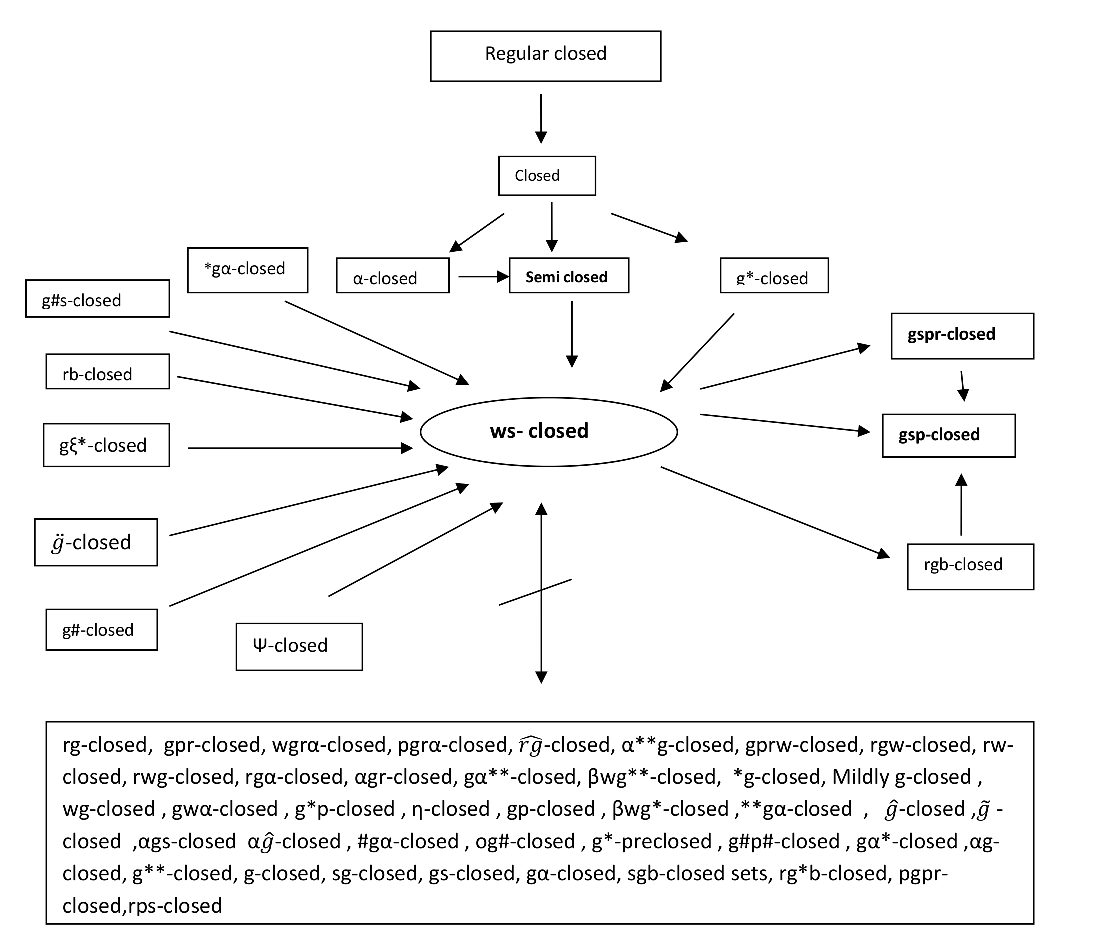
\includegraphics[scale=.75]{fig1.eps}
\end{figure}
\end{rem}

\begin{thm}\label{thm2.2.23}
The union of two ws-closed subsets of $\TSP$ is ws-closed.
\end{thm}

\begin{exm}\label{exm2.2.24}
Let $\TSP = \{1, 2, 3\}$ and $\tau = \{\phi, \TSP, \{1\}, \{2\}, \{1, 2\}\}$ thus the sets $\TSA= \{1\}$ and $\TSB= \{2\}$ are ws-$\TSC(\TSP)$ set but $\TSA\cup \TSB = \{1,2 \}$ is not a ws-$\TSC(\TSP)$.
\end{exm}

\begin{thm}\label{thm2.2.25}
The intersection of two ws-closed subsets of $\TSP$ is ws-closed.
\end{thm}

\begin{proof}
Take up $\clrD$ and $\TSE\in \ws$-$\TSC(\TSP)$. Let $\TSU$ be any semiopen set $\in\TSP \ni: (\clrD\cap \TSE)\subseteq \TSU$ that is $\clrD\subseteq \TSU$ and $E\subseteq \TSU$. Since $\clrD$ and $\TSE$ are ws-$\TSC(\TSP)$ then $\scl(\clrD) \subseteq  \TSU$ and $\scl(\TSE)\subseteq \TSU$ and we know that $(\scl(\clrD)\cap \scl(\TSE)) = \scl(\TSD\cap \TSE)\subseteq \TSU$. Therefore $\clrD\TSE$ is ws-closed in $\TSP$.
\end{proof}

\begin{thm}\label{thm2.2.26}
Assuming subset $\clrD$ of a topological space $\TSP$ is ws-$\TSC(\TSP)$ then $\scl(\clrD)-\clrD~\cancel{\exists}$ any non-empty open set in $\TSP$ but inverse is untrue.
\end{thm}

\begin{proof}
Take up $\clrD\in\ws$-$\TSC(\TSP)$ and Pretend $\TSF$ be an non empty w-$\TSC(\TSP)$ subset of $\scl(\clrD)$-$\clrD$. $\TSF\subseteq \scl(\clrD)-\clrD\Rightarrow\TSF\subseteq \scl(\clrD)\cap(\TSP-\clrD)\Rightarrow \TSF\subseteq \scl(\clrD)$ $\to$ (1) \& $\TSF\subseteq\TSP-\clrD$

$\Rightarrow \clrD\subseteq \TSP-\TSF$ and $\TSP-\TSF$ is w-open set and $\clrD$ is an ws-$\TSC(\TSP)$, $\scl(\clrD)\subseteq \TSP-\TSF$

$\Rightarrow \TSF\subseteq \TSP-\scl(\clrD)$ $\to$ (2) from equations (1) and (2) we get $\TSF\subseteq \scl(\clrD)\cap(\TSP-\scl(\clrD))=\emptyset$

$\Rightarrow\TSF =\Phi$ thus $\scl(\clrD)-\clrD$ will not contain any non-empty w-$\TSC(\TSP)$.

We use example \ref{exam2.2.27} to prove the inverse of theorem is untrue.
\end{proof}

\begin{exm}\label{exam2.2.27}
Take $\TSP=\{1,2,3,4\}$, $\tau=\{\TSP,\phi,\{1\},\{1, 2\},\{1,2,3\}\}$ then the set $\clrD=\{1\}$ $\scl\{1\}=\{1,2,3\}$, $\scl\{\clrD\}-\clrD=\{2,3\}\cancel{\exists}$ any non-empty w-$\TSC(\TSP)$ but $\clrD$ is not ws-$\TSC(\TSP)$.
\end{exm}

\begin{thm}\label{thm2.2.28}
If $\clrD\in\ws$-$\TSC(\TSP)$ and $\clrD\subseteq \TSE\subseteq \scl(\clrD)$ then $\TSE$ is also ws-$\TSC(\TSP)$.
\end{thm}

\begin{proof}
Take up $\clrD\in \ws$-$\TSC(\TSP)$, $\ni: \TSE\subseteq \scl(\clrD)$. Assume $\TSU$ be a w-open set of $\TSP \ni: \TSE\subseteq \TSU$ then $\clrD\subseteq \TSU$. Since $\clrD$ is ws-$\TSC(\TSP)$ we have $\scl(\clrD)\subseteq \TSU$ and $\clrD\subseteq \TSU$. Now $\TSE\subseteq \scl(\clrD)\Rightarrow\scl(\TSE)\subseteq \scl(\scl(\clrD))=\scl(\clrD)\subseteq \TSU$. That is $\scl(\TSE)\subseteq \TSU$. Therefore $\TSE$ is a ws-$\TSC(\TSP)$.
\end{proof}

We use example \ref{exam2.2.29} to prove the inverse of theorem is untrue.

\begin{exm}\label{exam2.2.29}
Take up $\TSP = \{1,2,3 \}$, $\tau = \{\phi, \TSP, \{1\}, \{2\}, \{1, 2\}\}$ then the set $\clrD=\{1\}$, $\TSE=\{1,3\}\ni:\clrD$ and $\TSE$ are ws-$\TSC(\TSP)$ but $\clrD\subseteq \TSE \not\subseteq\scl(\clrD)$ because $\scl(\clrD)=\{1\}$.
\end{exm}

\begin{thm}\label{thm2.2.30}
Pretend $(\TSP,\tau)$ is a topological space then $\forall x$ belongs to $\TSP$ the set $\TSP-\{\TSx\}$ is ws-$\TSC(\TSP)$ or semi open.
\end{thm}

\begin{proof}
Let $\TSx\in\TSP$. Suppose $\TSP-\{\TSx\}\not\in$ semiopen set. Then $\TSP$ is the only semiopen set containing $\TSP-\{\TSx\}$ that is $\TSP-{\TSx} \subseteq \TSP\Rightarrow \cl(\TSP-\{\TSx\}) \subseteq \cl(\TSP)\Rightarrow \cl(\TSP-\{\TSx\})\subseteq \TSP$. Therefore $\TSP-\{\TSx\}$ is ws-$\TSC(\TSP)$.
\end{proof}

\begin{thm}\label{thm2.2.31}
Take up $\clrD\in \ws$-$\TSC(\TSP)$. Then $\clrD$ is semi-closed iff $\scl(\clrD)-\clrD$ is w-open.
\end{thm}

\begin{proof}
Necessity: Pretend $\clrD$ is g-$\TSC(\TSP)$. Then $\scl(\clrD)=\clrD$ that is $\scl(\clrD)-\clrD=\phi$ which is w-open set in $\TSP$.

Sufficiency: Pretend $\clrD$ is ws-$\TSC(\TSP)$ and $\scl(\clrD)-\clrD$ is w-open, By the Theorem \ref{thm2.2.26} $\scl(\clrD)-\clrD=\phi\Rightarrow \scl(\clrD)=\clrD$. Therefore $\clrD$ is semi-$\TSC(\TSP)$.
\end{proof}

\begin{thm}\label{thm2.2.32}
Let $\clrD\subseteq \TSQ\subseteq \TSP$ and Pretend that $\clrD$ is ws-$\TSC(\TSP)$. Then $\clrD$ is ws-closed relative to $\TSY$.
\end{thm}

\begin{proof}
Let $\clrD\subseteq \TSQ\cap \TSG$ where $\TSG$ is w-open. Since $\clrD$ is ws-$\TSC(\TSP)$, then $\clrD\subseteq \TSG$ and $\scl(\clrD)\subseteq \TSG$. This
implies that $\TSQ \cap \scl(\clrD) \subseteq \TSQ\cap \TSG$ where $\TSQ \cap \scl(\clrD)$ is closed set of $\clrD$ in $\TSQ$. Thus $\clrD$ is ws-closed
relative to $\TSQ$.
\end{proof}

\begin{thm}\label{thm2.2.33}
In a topological space $\TSP$ if $\SO(\TSP) =\{\TSP, \phi\}$ then each subset $\TSP$ is a ws-$\TSC(\TSP)$.
\end{thm}

\begin{proof}
Take up $\TSP$ be a topological space and $\SO(\TSP)=\{\TSP, \phi\}$. Let $\clrD$ be any subset of $\TSP$. Pretend $\clrD=\phi$. Then $\phi$ is ws-$\TSC(\TSP)$. Pretend $\clrD\neq\phi$. Then $\TSP$  is the only semiopen set containing $\TSA$ and so $\scl(\clrD)\subseteq \TSP$. Hence $\clrD$ is ws-$\TSC(\TSP)$. 

We use example \ref{exam2.2.34} to prove the inverse of theorem is untrue.
\end{proof}

\begin{exm}\label{exam2.2.34}
Let $\TSP  = \{1, 2, 3\}$, $\tau = \{\phi, \TSP, \{1\}, \{2, 3\}\}$. Then each subset of $(\TSP,\tau)$ is a ws-$\TSC(\TSP)$, but $\SO(\TSP)= \{\phi, \TSP, \{1\}, \{2, 3\}\}$.
\end{exm}

\begin{thm}\label{thm2.2.35}
If $\clrD\in$ regular open and gspr-closed then $\clrD\in\ws$-$\TSC(\TSP)$.
\end{thm}

\begin{proof}
Take up $\clrD\in$ regular open and gspr-closed in $\TSP$. Let $\TSM$ be any w-open set in $\TSP\ni: \clrD\subseteq \TSM$. Since $\clrD$ is regular open and gspr-closed, by definition, $\scl(\clrD)\subseteq \clrD$ then $\scl(\clrD)\subseteq \clrD\subseteq \TSU$. Hence $\clrD$ is ws-$\TSC(\TSP)$.
\end{proof}

\begin{thm}\label{thm2.2.36}
If $\clrD\in$ regular open and rgb-closed then $\clrD\in$ ws-$\TSC(\TSP)$.
\end{thm}

\begin{proof}
Take up $\clrD$ be regular open and rgb-closed in $\TSP$. Let $\TSM$ be any w-open set in $\TSP$. $\ni: \clrD\subseteq \TSM$. Seeing that $\clrD$ is regular open and rgb-closed in $\TSP$, by definition, $\scl(\clrD)\subseteq \clrD$ thus $\scl(\clrD)\subseteq \clrD\subseteq \TSM$. Hence $\clrD$ is ws-$\TSC(\TSP)$.
\end{proof}

\begin{thm}\label{thm2.2.37}
If $\clrD\in$ semiopen and swg*-closed then $\clrD\in\ws$-$\TSC(\TSP)$.
\end{thm}

\begin{proof}
Let $\clrD\in$ semiopen and swg*-closed in $\TSP$. Let $\TSM$ be any w-open set in $\TSP \ni: \clrD\subseteq \TSM$. Since $\clrD$ is semiopen and swg*-closed in $\TSP$, by definition, $\scl(\clrD)\subseteq \clrD$ thus $\scl(\clrD)\subseteq \clrD\subseteq \TSM$. Hence $\clrD$ is ws-$\TSC(\TSP)$.
\end{proof}

\begin{thm}\label{thm2.2.38}
If $\clrD\in$ is semiopen and swg-closed then $\clrD\in\ws$-$\TSC(\TSP)$.
\end{thm}

\begin{proof}
Take up $\clrD$ be semiopen and swg-closed in $\TSP$. Let $\TSM$ be any w-open set in $\TSP\ni : \clrD\subseteq \TSM$. Since $\clrD$ is semiopen and swg-closed in $\TSP$, by definition, $\scl(\clrD)\subseteq \clrD$ implies $\scl(\clrD)\subseteq \clrD\subseteq \TSM$. Hence $\clrD$ is ws-$\TSC(\TSP)$.
\end{proof}

\begin{thm}\label{2.2.39}
If $\clrD\in$ is semiopen and sg-closed then $\clrD\in\ws$-$\TSC(\TSP)$.
\end{thm}

\begin{proof}
Take up $\clrD$ be semiopen and sg-closed in $\TSP$. Let $\TSM$ be any w-open set in $\TSP \ni: \clrD\subseteq \TSM$. Since $\clrD$ is semiopen and sg-closed in $\TSP$, by definition, $\scl(\clrD)\subseteq \clrD$ implies $\scl(\clrD)\subseteq \clrD\subseteq \TSM$. Hence $\clrD$ is ws-$\TSC(\TSP)$.
\end{proof}

\begin{thm}\label{thm2.2.40}
If $\clrD\in$ semiopen and sgb-closed then $\clrD\in\ws$-$\TSC(\TSP)$.
\end{thm}

\begin{proof}
Take up $\clrD$ be semiopen and sgb-closed in $\TSP$. Let $\TSM$ be any w-open set in $\TSP \ni: \clrD\subseteq \TSM$. Since $\clrD$ is semiopen and sgb-closed in $\TSP$, by definition, $\scl(\clrD)\subseteq \clrD$ implies $\scl(\clrD)\subseteq \clrD\subseteq \TSM$. Hence $\clrD$ is ws-$\TSC(\TSP)$.
\end{proof}

\begin{thm}\label{thm2.2.41}
If $\clrD\in$ semiopen and $\alpha$gs-closed then $\clrD\in\ws$-$\TSC(\TSP)$.
\end{thm}

\begin{proof}
Take up $\clrD\in$ semiopen and $\alpha$gs-closed in $\TSP$. Let $\TSM$ be any w-open set in $\TSP\ni : \clrD\subseteq \TSM$. Since $\clrD$ is semiopen and $\alpha$gs-closed in $\TSP$, by definition, $\scl(\clrD)\subseteq \clrD$ implies $\scl(\clrD)\subseteq \clrD\subseteq \TSM$. Hence $\clrD$ is ws-$\TSC(\TSP)$.
\end{proof}

\begin{thm}\label{thm2.2.42}
If $\clrD\in\beta$-open and $\beta$wg*-closed then $\clrD\in\ws$-$\TSC(\TSP)$.
\end{thm}

\begin{proof}
Let $\clrD\in\beta$-open and $\beta$wg*-closed in $\TSP$. Let $\TSM$ be any regular semiopen set in $\TSP\ni : \clrD\subseteq \TSM$. Since $\clrD$ is $\beta$-open and $\beta$wg*-closed in $\TSP$, by definition, $\gcl(\clrD)\subseteq \clrD$ implies $\gcl(\clrD)\subseteq \clrD\subseteq \TSM$. Hence $\clrD$ is ws-closed in $\TSP$.
\end{proof}

\begin{thm}\label{thm2.2.43}
If $\clrD\in$ both open and g-closed then $\clrD\in$ ws-$\TSC(\TSP)$.
\end{thm}

\begin{proof}
Let $\clrD\in$ open and g-closed in $\TSP$. Let $\TSM$ be any regular open set in $\TSP\ni \clrD\subseteq \TSM$. by definition, $\cl(\clrD)\subseteq \clrD\subseteq \TSM$ and $\gcl(\clrD)=\clrD$. This implies $\cl(\clrD)\subseteq \gcl(\clrD) \subseteq \clrD\subseteq \TSM\Rightarrow\gcl(\clrD)\subseteq \TSM$. Hence $\clrD$ is ws-$\TSC(\TSP)$.
\end{proof}

\begin{thm}\label{thm2.2.44}
If $\clrD\in$ regular semiopen and rw-closed then $\clrD\in\ws$-$\TSC(\TSP)$.
\end{thm}

\begin{proof}
Take up $\clrD\in$ regular semiopen and rw-$\TSC(\TSP)$ in $\TSP$. Let $\TSM$ be any w-open set in $\TSP\ni: \clrD\subseteq \TSM$. Now $\clrD\subseteq \clrD$ by hypothesis $\cl(\clrD)\subseteq \clrD$ then we know that $\cl(\clrD) \subseteq \scl(\clrD)\subseteq \clrD$. Hence $\scl(\clrD)\subseteq \TSM$ therefore $\clrD$ is ws-$\TSC(\TSP)$.
\end{proof}

\begin{thm}\label{thm2.2.45}
If $\clrD\in$ regular semiopen and R*-closed then $\clrD\in\ws$-$\TSC(\TSP)$.
\end{thm}

\begin{proof}
Take up $\clrD\in$ regular semiopen and R*-closed in $\TSP$. Let $\TSM$ be any w-open set in $\TSP \ni:\clrD\subseteq \TSM$. Now $\clrD\subseteq \clrD$ by hypothesis $\cl(\clrD)\subseteq \clrD$ then we know that $\cl(\clrD) \subseteq \scl(\clrD)\subseteq \clrD$. Hence $\scl(\clrD)\subseteq \TSM$ therefore $\clrD$ is ws-$\TSC(\TSP)$.
\end{proof}

\begin{thm}\label{thm2.2.46}
If $\clrD\in$ regular semiopen and gprw-closed then $\clrD\in$ ws-$\TSC(\TSP)$.
\end{thm}

\begin{proof}
Take up $\clrD$ be regular semiopen and gprw-closed in $\TSP$. Let $\TSM$ be any w-open set in $\TSP\ni : \clrD\subseteq \TSM$. Now $\clrD\subseteq \clrD$ by hypothesis $\cl(\clrD)\subseteq \clrD$ then we know that $\cl(\clrD) \subseteq \scl(\clrD)\subseteq \clrD$. Hence $\scl(\clrD)\subseteq \TSM$ therefore $\clrD$ is ws-$\TSC(\TSP)$.
\end{proof}

\begin{thm}\label{thm2.2.47}
If $\clrD\in$ is regular semiopen and rgw-closed then $\clrD\in\ws$-$\TSC(\TSP)$.
\end{thm}

\begin{proof}
Take up $\clrD$ be regular semiopen and rgw-closed in $\TSP$. Let $\TSM$ be any w-open set in $\TSP \ni: \clrD\subseteq \TSM$. Now $\clrD\subseteq \clrD$ by hypothesis $\cl(\clrD)\subseteq \clrD$ then we know that $\cl(\clrD) \subseteq \scl(\clrD)\subseteq \clrD$. Hence $\scl(\clrD)\subseteq \TSM$ therefore $\clrD$ is ws-$\TSC(\TSP)$ .
\end{proof}

\section{ws-open sets in topological spaces}

\begin{dfn}\label{defi2.3.1}
A subset $\clrD$ of a topological space $(\TSP,\tau)$ is called a ws-open set in $\TSP$ if $\clrD^{\text{c}}$ is a ws-closed.
\end{dfn}

\begin{thm}\label{thm2.3.2}
For any topological space $(\TSP,\tau)$ we have the following
\begin{enumerate}[(i)]
\item Each regular (respectively, semi, $\alpha$, g$^{\#}$, *g$\alpha$, g\#s, rb, $\ddot{g}$, g$\xi$*, $\alpha$gp, $\psi$) open set in $\TSP$ is ws-open in $\TSP$.
\item Each ws-open set in $\TSP$ is gspr (respectively gsp, rgb) open set in $\TSP$.
\end{enumerate}
\end{thm}

\begin{thm}\label{thm2.3.3}
If $\clrD$ and $\TSE$  are ws-open sets in space $\TSP$ then $\clrD\cup \TSE$  is also a ws-open set in $\TSP$.
\end{thm}

\begin{proof}
Take up $\clrD$ and $\TSE$ be ws-open sets in $\TSP$. Then $\clrD^{\text{c}}$ and $\TSE^{\text{c}}$ are ws-$\TSC(\TSP)$, by Theorem \ref{thm2.2.27} $\clrD^{\text{c}} \cap E^{\text{c}}$ is also ws-$\TSC(\TSP)$. That is $\clrD^{\text{c}} \cap \TSE^{\text{c}} = (\TSA\cup \TSE)^{\text{c}}$ is ws-$\TSC(\TSP)$. Therefore $(\TSA\cup \TSE)$ is ws-open set in $\TSP$.
\end{proof}

\begin{rem}\label{rem2.3.4}
Intersection of ws-open sets in $\TSP$ is not a ws-open set in $\TSP$.
\end{rem}

\begin{exm}\label{exam2.3.5}
Take up $\TSP = \{1,2, 3\}$, $\tau = \{\phi, \TSP, \{1\}, \{2\}, \{1, 2\}\}$. ws-open $= \{\phi, \TSP, \{1\}, \{2\}, \{1, 2\},\{1,3\},\{2,3\}\}$. If $\clrD= \{1,3\}$ and $\TSE=\{2,3\}$ then $\clrD$ and $\TSE$ are ws-open sets but $\TSA\cap \TSE=\{3\}$ is not a ws-open set in $\TSP$.
\end{exm}

\begin{thm}\label{thm2.3.6}
A subset $\clrD$ of a topological space $\TSP$ is ws-open iff $\TSM\subseteq  \text{ wsint } (\clrD)$ whenever $\TSM\subseteq \clrD$ and $\TSM$ is w-open in $\TSP$.
\end{thm}

\begin{proof}
Pretend $\clrD$ is ws-open. $\TSM\subseteq \clrD$ and $\TSM$ is w-open. Then $\clrD^{\text{c}} \subseteq \TSM^{\text{c}}$ and $\TSM^{\text{c}}$ is also w-open. By the definition of ws-$\TSC(\TSP)$ $\scl(\clrD^{\text{c}})\subseteq \TSM^{\text{c}}$. But $\scl(\clrD^{\text{c}})=(\text{wsint}(\clrD))^{\text{c}}.=\TSP-\text{wsint}(\clrD)$ This implies $\TSM\subseteq \text{wsint}(\clrD)$ 

Inversely,

Suppose that $M\subseteq  \wsint(\clrD)$ whenever $\TSM\subseteq \clrD$, $\TSM$ is w-open in $\TSP$. Let $\clrD^{\text{c}} \subseteq \TSF$ where $\TSF$ is w-open in $\TSP$. $\TSF^{\text{c}} \subseteq \clrD$ and $\TSF^{\text{c}}$ is w-open in $\TSP$. we know that $F^{\text{c}} \subseteq \wsint(\clrD)$ and ($\wsint(\clrD))^{\text{c}} \subseteq \TSF$. Since $\scl(\clrD^{\text{c}})= (\wsint(\clrD))^{\text{c}}$ we have $\scl(\clrD^{\text{c}})\subseteq \TSM$. Thus $\clrD^{\text{c}}$ is ws-$\TSC(\TSP)$. That is $\clrD$ is ws-open set.
\end{proof}

\begin{thm}\label{thm2.3.7}
If $\sint(\clrD)\subseteq E\subseteq \clrD$ and $\clrD$ is ws-open set then $\TSE$ is ws-open set.
\end{thm}

\begin{proof}
Let $\sint(\clrD)\subseteq \TSE\subseteq \clrD$. Thus $\TSP-\clrD\subseteq \TSP-\TSE\subseteq \TSP-\sint(\clrD)$. That is $\TSP-\clrD\subseteq \TSP-\TSE\subseteq \scl(\TSP-\clrD)$, since $\TSP-\clrD$ is ws-$\TSC(\TSP)$ and also $\TSP-\TSE$ is ws-$\TSC(\TSP)$. Therefore $\TSE$  is ws-open set.
\end{proof}

\section{ws-Closure in topological spaces}\label{sec2.4}

\begin{dfn}\label{defi2.4.1} 
For a subset $\clrD$ of $(\TSP, \tau)$, ws-closure of $\clrD$ is denoted by $\wscl(\clrD)$ and it is defined as $\wscl(\clrD)=\cap \{\TSG: \clrD\subseteq \TSG, \TSG\subseteq \ws\TSC(\TSP)\}$ or intersection of all ws-$\TSC(\TSP)$s containing $\clrD$.
\end{dfn}

\begin{thm}\label{thm2.4.2}
If $\clrD$ and $\TSE$  are subsets of space $(\TSP, \tau)$ then
\begin{enumerate}[(i)]
\item $\wscl(\TSP)=\TSP$, $\wscl(\phi)=\phi$
\item $\clrD\subseteq \wscl(\clrD)$
\item if $\TSE$ is any ws-$\TSC(\TSP)$ containing $\clrD$ then $\wscl(\clrD)\subseteq \TSE$
\item If $\clrD\subseteq \TSE$ then $\wscl(\clrD)\subseteq \wscl(\TSE)$
\item $\wscl(\clrD)=\wscl(\wscl(\clrD))$
\item $\wscl(\clrD\cup \TSE)=(\wscl(\clrD)\cup \wscl(\TSE))$
\end{enumerate}
\end{thm}

\begin{proof}
\begin{enumerate}[(i)]
\item From ws-closure defination, $\wscl(\TSP)$ =Intersection of all ws-$\TSC(\TSP)$ containing $\TSP =\TSP \cap \ws$-$\TSC(\TSP)$ containing $\TSP=\TSP\cap \TSP =\TSP$, Therefore $\wscl(\TSP)=\TSP$. By the definition of ws-closure, $\wscl(\phi)$=intersection of all ws-$\TSC(\TSP)$s containing $\phi =\phi\cap$  any ws-$\TSC(\TSP)$ containing $\phi= \phi\cap \phi=\phi$. Therefore $\wscl(\phi)=\phi$.

\item By the definition of ws-closure of $\clrD$, it is obvious that $\clrD\subseteq  \wscl(\clrD)$.

\item Let $\TSE$ be any ws-$\TSC(\TSP)$ containing $\clrD$. Since $\wscl(\clrD)$ is the intersection of all ws-$\TSC(\TSP)$ containing $\clrD$. $\wscl(\clrD)$ is contained in each ws-$\TSC(\TSP)$ containing $\clrD$. Hence in particular $\wscl(\clrD)\subseteq \TSE$.

\item Let $\clrD$ and $\TSE$  be subsets of $(\TSP,\tau) \ni: \clrD\subseteq \TSE$. By the definition of ws-closure, $\wscl(\TSE)=\cap \{\TSF: \TSE\subseteq \TSF\in \wscl(\TSP)\}$. If $\TSE\subseteq \TSF\in \wscl(\TSP)$ then $\wscl(\TSE)\subseteq \TSF$. Since $\clrD\subseteq \TSE \subseteq \TSF\in \wscl(\TSP)$, we have $\wscl(\clrD)\subseteq \TSF$, $\wscl(\clrD)\subseteq \cap \{\TSF: \TSE\subseteq \TSF\in \wscl(\TSP)\}=\wscl(\TSE)$. Therefore $\wscl(\clrD)\subseteq \wscl(\TSE)$.

\item Let $\clrD$ be any subset of $\TSP$. By the definition of ws-closure, $\wscl(\clrD)=\cap \{\TSF: \TSA\subseteq \TSF \in \wscl(\TSP)\}$.

\item If $\clrD\subseteq \TSF\in \ws\TSC(\TSP)$ then $\wscl(\clrD)\subseteq \TSF$. Since $\TSF$ is a ws-$\TSC(\TSP)$ containing $\wscl(\clrD)$, by (iii) $\wscl(\wscl(\clrD))\subseteq \TSF$. Hence $\wscl(\wscl(\clrD))\subseteq \cap \{\TSF: \clrD\subseteq \TSF\in \wscl(\TSP)\}=\ws \TSC(\clrD)$. That is $\wscl(\wscl(\clrD))=\wscl(\clrD)$. Let $\clrD$ and $\TSE$  be subsets of $(\TSP,\tau)$. Clearly $\clrD\subseteq (\clrD\cup \TSE)$ and $\TSE\subseteq (\clrD\cup \TSE)$. From (iv) $(\wscl(\clrD)\cup \wscl(\TSE))\subseteq \wscl(\clrD\cup \TSE)$ ...(1) Now we need to determine that $\wscl(\clrD\cup \TSE)\subseteq \wscl(\clrD)\cup \wscl(\TSE)$. Suppose $P\not\in (\wscl(\clrD)\cup \wscl(\TSE))$ then their exists ws-closed sets $\clrD_{1}$ and $\TSE_{1}\ni: \clrD\subseteq \clrD_{1}$, $\TSE\subseteq \TSE_{1}$ and $\TSP\not\in (\clrD_{1} \cup \TSE_{1})$ Thus we have $(\clrD\cup \TSE)\subseteq (\clrD_{1} \cup \TSE_{1})$ and $(\clrD_{1} \cup \TSE_{1})$ is a ws-$\TSC(\TSP)$ by Theorem ... $\ni: P\not\in (\clrD_{1} \cup \TSE_{1})$. Thus $\TSP\not\in \wscl(\clrD\cup \TSE)$. Hence $\wscl(\clrD\cup \TSE)\subseteq (\wscl(\clrD)\cup \wscl(E))$ ....(2). From (1) and (2) we have $\wscl(\clrD\cup \TSE)=(\wscl(\clrD)\cup \wscl(\TSE))$.
\end{enumerate}
\end{proof}

\section{ws-Interior in topological space}

\begin{dfn}\label{defi2.4.3}
For a subset $\clrD$ of $(\TSP,\tau)$, ws-interior of $\clrD$ is denoted by $\wsint(\clrD)$ and it is defined as $\wsint(\clrD)= \cup \{\TSG: \TSG\subseteq \clrD$ and $\TSG$ is ws-open in $\TSP\}$ or $\cup \{\TSG: \TSG\subseteq \clrD$ and $\TSG \in \ws \TSO(\TSP)\}$ or $\wsint(\clrD)$ is the union of all ws-open sets contained in $\clrD$.
\end{dfn}

\begin{thm}\label{thm2.4.4}
Let $\clrD$ and $\TSE$  be subsets of space $\TSP$ then
\begin{enumerate}[(i)]
\item $\wsint (\TSP)=\TSP$, $\wsint(\phi)=\phi$
\item $\wsint(\clrD)\subseteq \clrD$
\item if $\TSE$ is any ws-open set contained in $\clrD$ then $E\subseteq \wsint(\clrD)$
\item If $\clrD\subseteq \TSE$ then $\wsint(\clrD)\subseteq \wsint(\TSE)$
\item $\wsint(\clrD)=\wsint(\wsint(\clrD))$
\item $\wsint(\clrD\cap \TSE)=(\wsint(\clrD)\cap \wsint(\TSE))$.
\end{enumerate}
\end{thm}

\begin{proof}
\begin{itemize}
\item[(i)] and (ii) follows by the definition of ws-interior of $\clrD$.
\item[(iii)] Let $\TSE$ is any ws-open set $\ni: \TSE\subseteq \clrD$. Let $\TSP\in\TSE$, $\TSE$  be ws-open set contained in $\clrD$, $\TSP$ is an interior point of $\clrD$ that is $\TSP\in \wsint(\clrD)$. Hence $\TSE\subseteq \wsint(\clrD)$.
\end{itemize}
similarly Proof of (iv), (v) and (vi) can be proved.
\end{proof}

\begin{thm}\label{thm2.4.5}
Pretend that a subset $\clrD$ of $\TSP$ is ws-open then $\wsint(\clrD)=\clrD$
\end{thm}

\begin{proof}
Take up $\clrD$ be ws-open set of $\TSP$. we know that $\wsint(\clrD)\subseteq \clrD \to (1)$ Also $\clrD$ is ws-open set contained in $\clrD$ from Theorem \ref{thm2.3.7} (iii) $\clrD\subseteq \wsint(\clrD)\to (2)$. Hence from (1) and (2) $\wsint(\clrD)=\clrD$.
\end{proof}

\begin{thm}\label{thm2.4.6}
If $\clrD$ and $\TSE$ are subsets of space $\TSP$ then $(\wsint(\clrD)\cup \wsint(\TSE))\subseteq \wsint(\clrD\cup \TSE)$
\end{thm}

\begin{proof}
As we know $\clrD\subseteq (\clrD\cup \TSE)$ and $\TSE\subseteq (\clrD\cup \TSE)$. We have Theorem \ref{thm2.3.7} (iv) $\wsint(\clrD)\subseteq \wsint(\clrD\cup \TSE)$ and $\wsint(\TSE)\subseteq \wsint(\clrD\cup \TSE)$. This implies that $\wsint(\clrD)\cup \wsint(\TSE)\subseteq \wsint(\clrD\cup \TSE)$.
\end{proof}


\section{ws-Neighbourhood of topological spaces}\label{sec2.5}

\begin{dfn}\label{defi2.5.1}
Let $(\TSP, \tau)$ is a topological space and $\TSx\in \TSP$, $\clrD$ subset $\TSN$ of $\TSP$ is termed to be ws-neighbourhood of $\TSx$ if $\exists$ ws-open set $\TSG \ni: \TSx\in \TSG\subseteq \TSN$
\end{dfn}

\begin{dfn}\label{defi2.5.2}
If $(\TSP, \tau)$ is a topological space and $\clrD$ be a subset of $\TSP$, a subset $\TSN$ of $\TSP$ is said to be ws-neighbourhood of $\clrD$ if their exists ws-open set $\TSG \ni: \clrD\subseteq \TSG\subseteq \TSN$.
\end{dfn}

\begin{dfn}\label{defi2.5.3}
The set of all ws-neighbourhood of $\TSx\in \TSP$ is called ws-neighbourhood system at $\TSx$ and it is indicated as ws-$\TSN(\TSP)$
\end{dfn}

\begin{thm}\label{thm2.5.4}
Each neighbourhood $\TSN$ of $\TSx\in \TSP$ is a ws-neighbourhood of~$\TSP$.
\end{thm}

\begin{proof}
Take up $\TSN$ be a neighbourhood of $\TSx\in \TSP$. To verify that $\TSN$ is a ws-neighbour\-hood of $\TSx$ by neighbourhood definition $\exists$ an open set $\TSG \ni: \TSx\in \TSG\subseteq \TSN$. Henceforth $\TSN$ is a ws-neighbourhood of $\TSx$.
\end{proof}

\begin{rem}\label{rem2.5.5} 
As usually, a ws-neighbourhood $\TSN$ of $\TSx$ belongs to $\TSP$ need not be a neighbourhood of $\TSx$ in $\TSP$.
\end{rem}

\section{ws-Limit points}\label{sec2.6}

\begin{dfn}\label{defi2.6.1}
Let $(\TSP, \tau)$ be a topological space and $\clrD$ be a subset of $\TSP$, then a point $\TSx\in \TSP$ is called a ws-limit point of $\clrD$ iff each ws-neighbourhood of $\TSx$ contains a point of $\clrD$ distinct from $\TSx$ that is $((\TSN-\{\TSx\})\cap \clrD)\neq \phi$ for each ws-neighbourhood $\TSN$ of $\TSx$.
\end{dfn}

Also equivalently Every ws-open set $\TSG$ containing $\TSx$ contains a point of $\clrD$ which is other than $\TSx$.

\begin{dfn}\label{defi2.6.2}
The set of all ws-limit points of the set $\clrD$ is termed a derived set $\clrD$ and is indicated by $\wsd(\clrD)$
\end{dfn}

\begin{thm}\label{thm2.6.3}
Each neighbourhood $\TSN$ of $\TSx$ belongs to $\TSP$ is a ws-neighbourhood of~$\TSP$.
\end{thm}

\begin{proof}
Take up $\TSN$ be a neighbourhood of $\TSx\in \TSP$. To verify that $\TSN$ is a ws-neighbour\-hood of $\TSx$ by the definition of neighbourhood $\exists$ an open set $\TSG \ni: \TSx\in\TSG\subseteq \TSN$. Henceforth $\TSN$ is a ws-neighbourhood of $\TSx$.
\end{proof}

\begin{rem}\label{rem2.6.4}
As usually, a ws-neighbourhood $\TSN$ of $\TSx$ belongs to $\TSP$ need not be a neighbourhod of $\TSx$ in $\TSP$ as seen from the following example.
\end{rem}

\begin{exm}\label{exam2.6.5}
Let $\TSP = \{1, 2, 3, 4 \}$, $\tau = \{\phi, \TSP, \{1\}, \{2\}, \{1, 2\}, \{1, 2, 3\}\}$. Then ws$\TSO(\TSP)= \{\phi, \TSP, \{1\}, \{2\}, \{3\}, \{4\},\{1, 2\},\{2, 3\}, \{3, 4\}, \{1, 2, 3\}\}$. The set $\{2, 3, 4\}$ is a ws-neighbourhood of the point $\{4\}$. Seeing that the ws-open set $\{3, 4\}$ is $\ni: \{4\}\subseteq \{3, 4\} \subseteq \{2, 3, 4\}$. However the set $\{2, 3, 4\}$ is not a neighbourhood of the point 4, since no open set $\TSG$ exists $\ni: 3\in \TSG\subseteq \{3, 4\}$
\end{exm}
